% Klassifiziert den Dokumenten-Typ
% Doku: http://exp1.fkp.physik.tu-darmstadt.de/tuddesign/
% Farben: http://www.tu-darmstadt.de/media/medien_stabsstelle_km/services/medien_cd/das_bild_der_tu_darmstadt.pdf
%  bigchapter: Chapter haben doppelte Schriftgröße
%  linedtoc: Linien im Inhaltsverzeichnis wie bei Überschriften
%  colorbacktitle: Der Dokumenten-Titel wird mir der Accentfarbe hinterlegt
\documentclass[bigchapter,colorback,accentcolor=tud4b,linedtoc,11pt]{tudreport}

% Input Dokument hat das Encoding UTF-8
\usepackage[utf8]{inputenc}
% Wichtiges Paket für Links und verlinktes Inhaltsverzeichnis
\usepackage{hhline}
\usepackage[ngerman]{hyperref}
% Paket für Fußnoten
\usepackage[stable]{footmisc}
% Paket für amsmath (aligned mathe formeln)
\usepackage{amsmath}
% Paket für Bibliotheks-Verzeichnis, square: Verwende eckige statt runde klammern
% \usepackage[square]{natbib}
% Paket zum Plotten von Datensätzen
\usepackage{pgfplots}
\usepgfplotslibrary{patchplots}


\pgfkeys{%
  /pgfplots/default/.style={%
    /pgf/number format/use comma,
    legend pos=north west,
    width=0.9\linewidth,
    height=0.7\linewidth,
    scale only axis,
    xmin=0,
    ymin=0,
    grid=both,
    tick align=outside,
    tickpos=left,
    minor x tick num=3,
    minor y tick num=4,
    minor grid style={dotted,thin},
    x tick label style={/pgf/number format/.cd,%
      set thousands separator={},
      set decimal separator={,}
    },%
    y tick label style={/pgf/number format/.cd,%
      set thousands separator={},
      set decimal separator={,}
    },%
  }
}

% Anhänge für Original-Messdaten
\usepackage{fancyvrb}

% redefine \VerbatimInput
\RecustomVerbatimCommand{\VerbatimInput}{VerbatimInput}%
{fontsize=\footnotesize,
 %
 frame=lines,  % top and bottom rule only
 framesep=2em, % separation between frame and text
 fontsize=\scriptsize,
 %
 labelposition=topline,
 %
 commandchars=\|\(\), % escape character and argument delimiters for
                      % commands within the verbatim
 commentchar=*        % comment character
}

% Polar Plots
\usetikzlibrary{pgfplots.polar}
% Verwende deutsche Bezeichner für Inhaltsverzeichnis, ... (ngerman = New German: neue Rechtschreibung)
\usepackage{ngerman}
% Deutsche Zahlen (entfernt z.B. das Leerzeichen nach einem Dezimal-Komma)
\usepackage{ziffer} 

\usepackage[verbose]{placeins}

%wegen Grafikverschiebung hinzugefügt
\usepackage{float}

%\usepackage{graphicx}
%\usepackage{caption}
\usepackage{subcaption} %Für subfigures

% PDF-Optionen
\hypersetup{%
  pdftitle={TU Darmstadt \- Physikalisches Praktikum für Fortgeschrittene},
  pdfauthor={Esra Bauer und Sören Link},
  pdfsubject={Versuch 5.4},
  pdfview=FitH,
}
% Nummeriere formeln in Subsections einzeln
% Kleines makro zur assymetrischen Fehlerangabe

% Entspricht-Zeichen
\usepackage{scalerel}

\newcommand\equalhat{%
\let\savearraystretch\arraystretch
\renewcommand\arraystretch{0.3}
\begin{array}{c}
\stretchto{
    \scalerel*[\widthof{=}]{\wedge}
    {\rule{1ex}{3ex}}%
}{0.5ex}\\ 
=%
\end{array}
\let\arraystretch\savearraystretch
}
%BEGINN TITELSEITE

\title{Tieftemperatur Messung an Suprafluidem Helium}

\subtitle{Esra Bauer (1906093) \\Sören Link {1582378}}

\subsubtitle{Betreuer:Michael Lannert \hfill Versuchsdatum: 1. Juni 2015}

\author{Esra Bauer, Sören Link}

%\settitlepicture{img/title.jpg}

\institution{Physikalisches Praktikum \\für Fortgeschrittene \\ Versuch 5.4}

\date{\today}


%ENDE TITELSEITE

\begin{document}
%ANFANG DOKUMENT

%Titelseite einfügen
\maketitle

%Inhaltsverzeichnis einfügen
\tableofcontents

%ANFANG INHALT

\chapter{Einleitung}

\chapter{Grundlagen}

\section{Primäre und sekundäre Thermometer}

\section{Kühlverfahren zum Erreichen tiefer Temperaturen}

\section{Der $\lambda$-Punkt}

\section{Curie- und Curie-Weiss-Gesetz}

\subsection{Herleitung des Curie-Gesetzes}

\begin{align*}
E(x,y) &= t \cdot U^*(x,y) U(x,y) \\
       &= t \cdot \left( |A_0|^2 + |A_1(x,y)|^2 + A_0 A_1(x,y) e^{-i \phi (x,y) -ax} + A_0 A_1(x,y) e^{i \phi (x,y) -ax} \right) \\
       &= t \cdot \left( |A_0|^2 + |A_1(x,y)|^2 + A_0 A_1(x,y) cos(\phi (x,y) -ax) \right)
\end{align*}

\chapter{Versuchsaufbau}

\chapter{Versuchsdurchführung und Auswertung}

\section{Temperatur am Probenort}

\section{Eichung des sekundären Thermometers}

\begin{figure}[H]
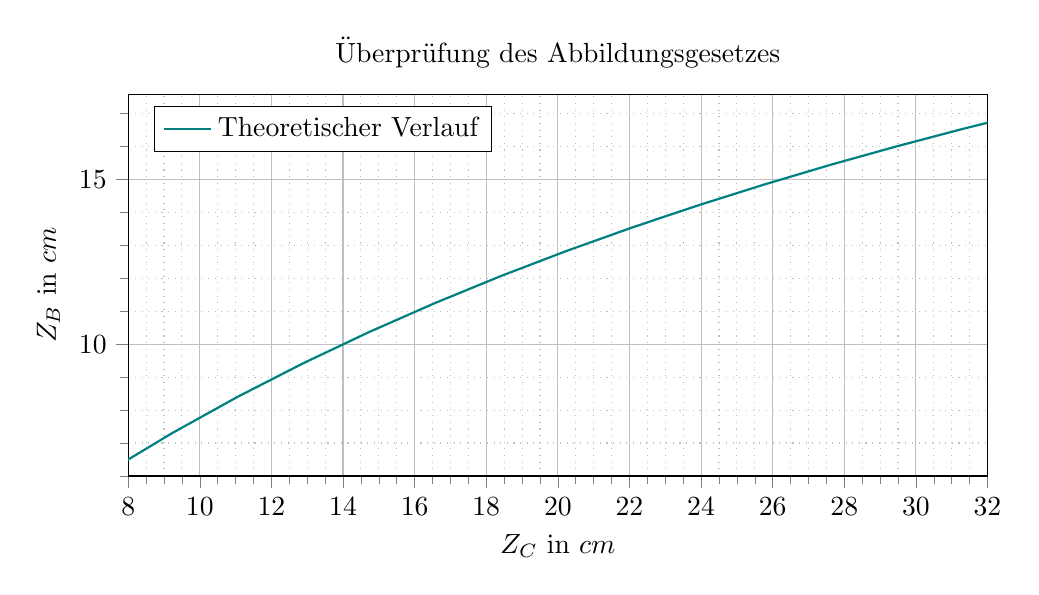
\begin{tikzpicture}
\begin{axis}[
  default,
  title={Überprüfung des Abbildungsgesetzes},
  xlabel=$Z_C$ in $cm$,
  ylabel=$Z_B$ in $cm$,
  xmin=8,
  xmax=32,
  ymin=6,
  height=0.4\linewidth,
]
\addplot[teal, thick, mark=x, mark size=0pt, samples=20, domain=-0:35] {(1/35+1/x)^(-1)};
\addlegendentry{Theoretischer Verlauf}
\end{axis}
\end{tikzpicture}
    \caption{Gemessene Werte für die Bildweite sowie der theoretische
      Verlauf. Die Theorie deckt sich hier sehr gut mit den
      aufgenommenen Daten.}
\end{figure}

\section{Bestimmung des $\lambda$-Punktes}

\section{Energiebetrachtung}

\chapter{Fazit}


%ENDE INHALT
\cleardoublepage{}
% Eintrag fürs Inhaltsverzeichnis
\newpage
\begin{thebibliography}{100}
  \bibitem{anleitung} Versuchsanleitung zum Versuch Tieftemperatur Messung an Suprafluidem Helium, heruntergeladen am 05.06.2015 von der Homepage des IAP der TU Darmstadt
\end{thebibliography}
\end{document}

%%% Local Variables:
%%% mode: latex
%%% TeX-master: t
%%% End:
